%!TEX root = main.tex
\subsection{Introduction}
To improve the reliability of the channel, Low Density Parity Check (LDPC) is implemented in this part. Its aim is to add redundancy to the information sent by the transmitter and use these additional bits to detect and correct errors. Besides, the parity check matrix used with LDPC has a small numbers of non-zero elements and allows a lower complexity of its implementation.
\subsection{LDPC encoding and hard decoding}
Figure~\ref{fig:ldpcBER} illustrates the channel coding gain as a function of the number of iterations.
In the rest of this section, the information bits are coded using (256,128) LDPC.
\begin{figure}[htbp]
    \centering
    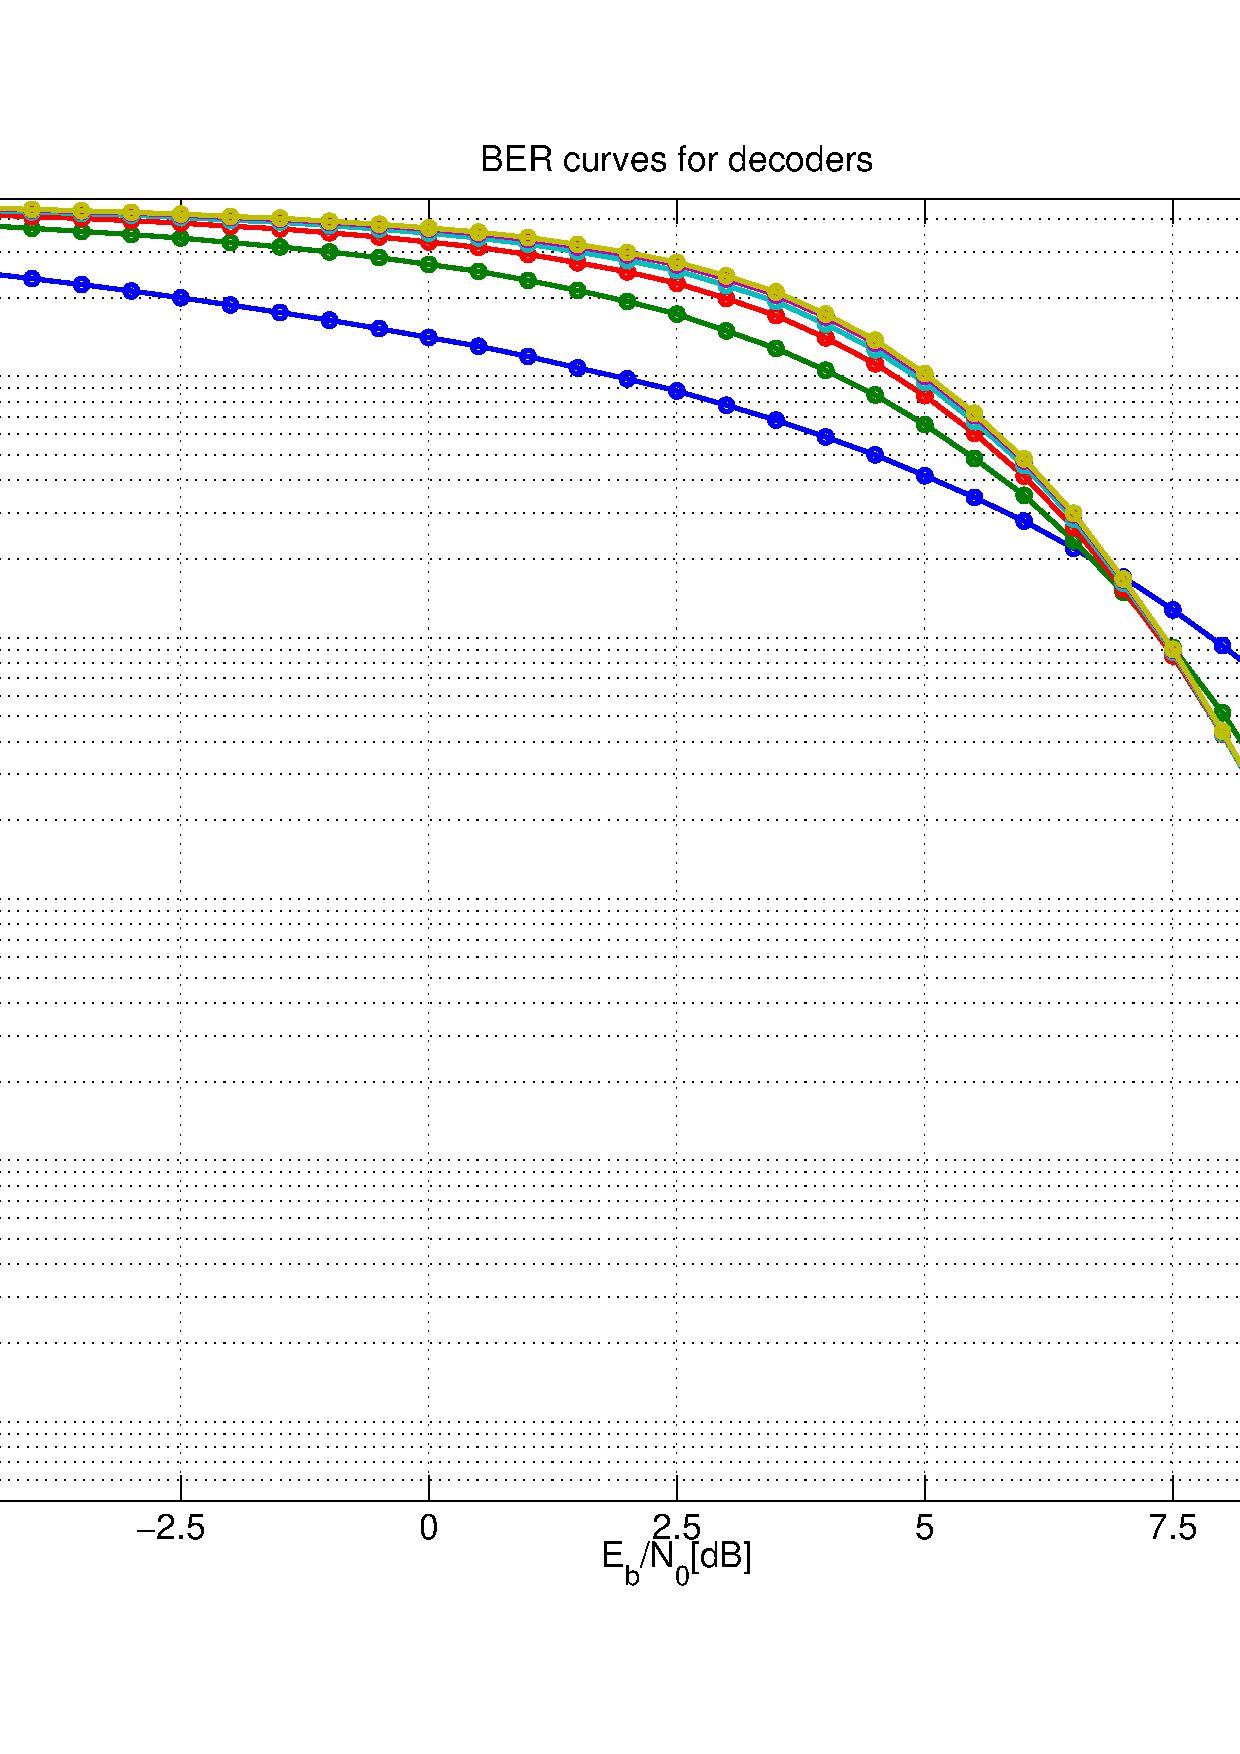
\includegraphics[width=\textwidth]{ldpcBER4.pdf}
    \caption{BER curves for different number of hard decoding iterations, compared with previous results.\label{fig:ldpcBER}}
\end{figure}

\subsection{Soft decoding}
Figure~\ref{fig:sldpcBER} compares the BER curves for the channel without coding, with coding and hard decoding and with different number of soft decoding iterations.
\begin{figure}[htbp]
    \centering
    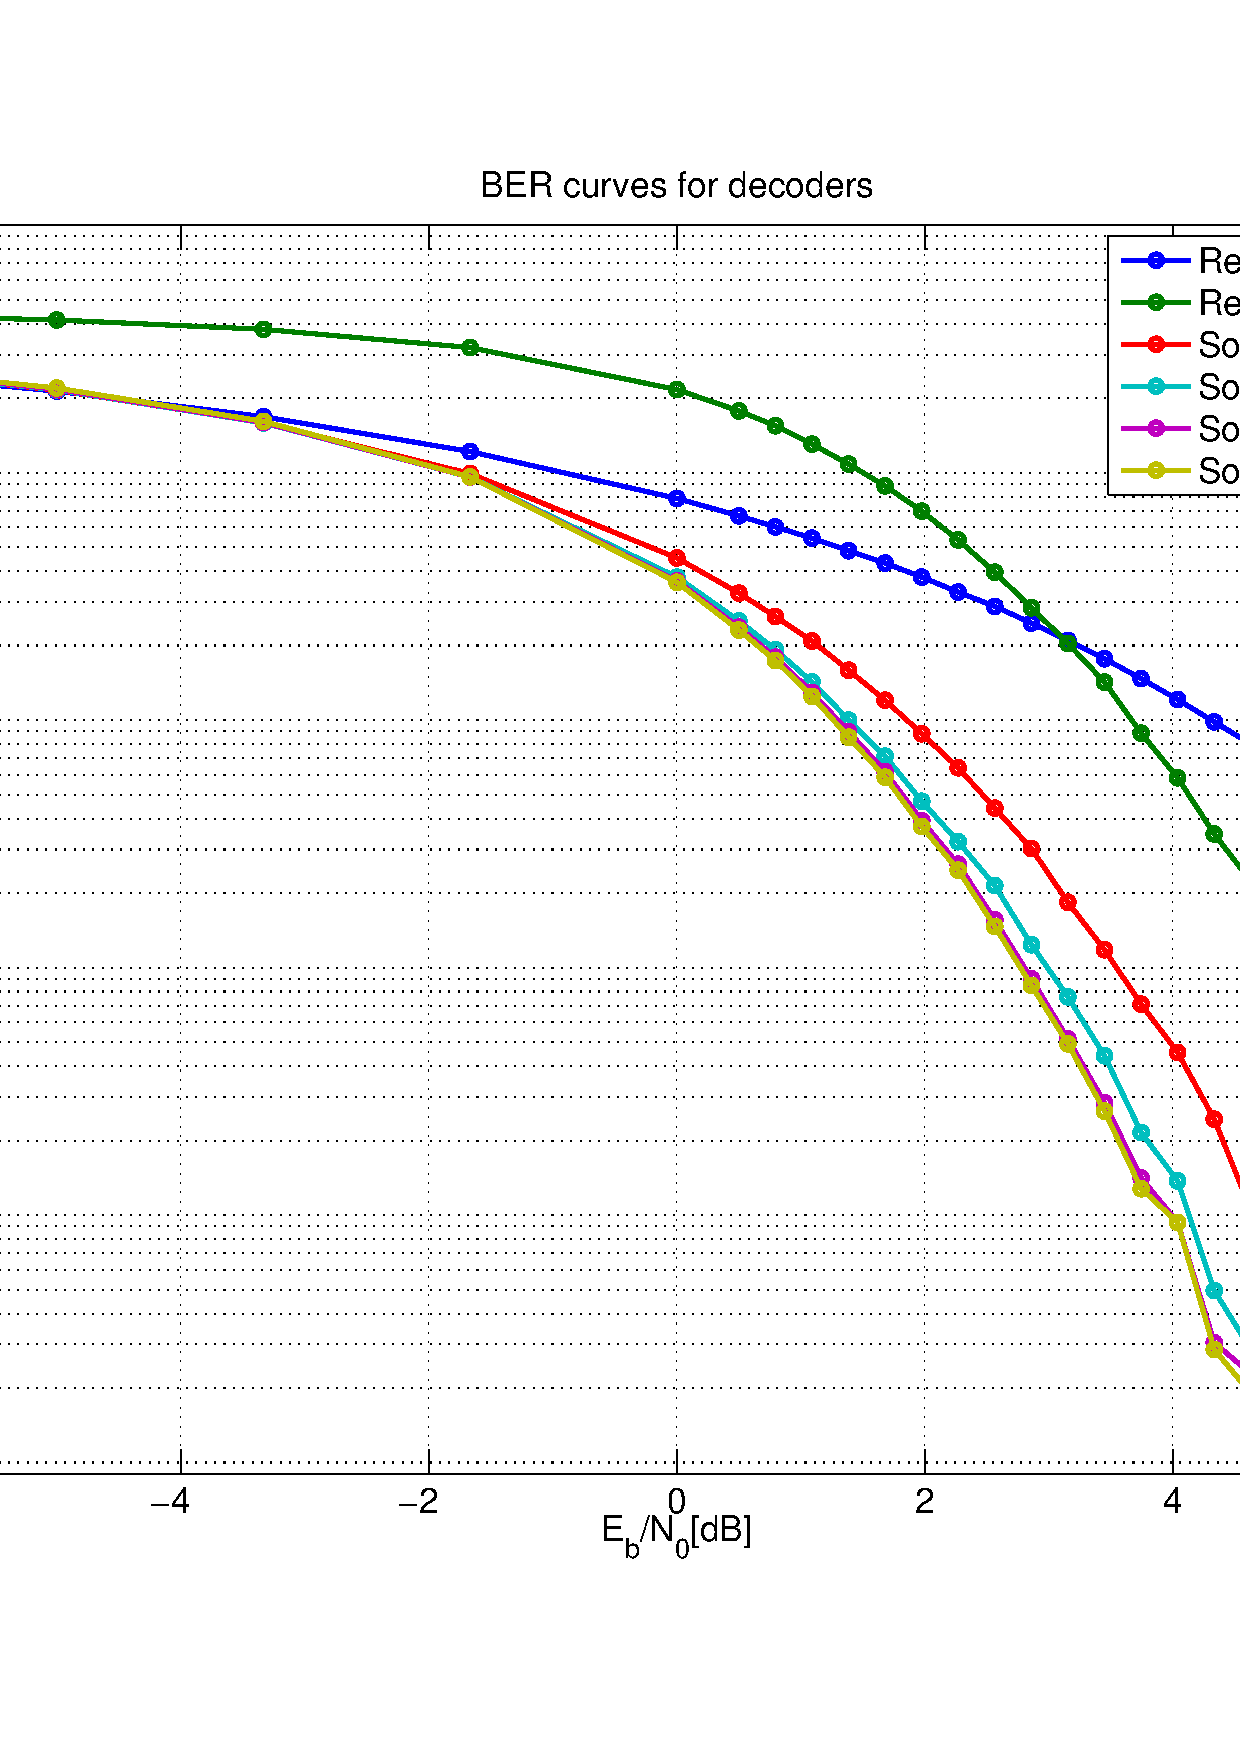
\includegraphics[width=\textwidth]{sldpcBER5.pdf}
    \caption{BER curves for different number of soft decoding iterations, compared with hard decoding and no coding.\label{fig:sldpcBER}}
\end{figure}
As will be explained in the next subsection, BPSK is used for this experiment.

\subsection{Questions}
\subsubsection{Simulation}
\paragraph{When building the new BER curves, do you consider the uncoded or coded bit energy on the x-axis?}
Here we consider the coded bit energy on the x-axis, but both options are interesting.
In a low-power application, the relevant metric is energy spent per sent bit of information in order to achieve a given error rate, which means the uncoded bit energy should be used on the x-axis.
If the emitter has constant power, the relevant metric is the coded bit energy which is defined as $\frac{P}{f_m \cdot \log_2(N_{sym})}$.

\paragraph{How do you limit the number of decoder iteration}
For hard decoding, the decoding stops as soon as one decoding iteration does not update the coded block, or when the maximum number of iterations is reached. This maximum number of iteration is set to 5. Figure~\ref{fig:ldpcBER} shows that very few additional errors are corrected past this value.
For soft decoding, the decoding stops as soon as there are no more detected errors, or when an iteration has actually introduced errors, or when the maximum number of iterations is reached.

\paragraph{Why is it much simpler to implement the soft decoder for BPSK or QPSK than for 16-QAM or 64-QAM?}